\section{Задание 1}

Ликвидируйте перегрузку ресурсов в проекте.

В данный момент в проекте наблядается перегрузка 3 ресурсов:
\begin{enumerate}
	\item Системный аналитик;
	\item Художник;
	\item Технический писатель;
\end{enumerate}

Перегрузка произошла из за одновременного выполняния задач.

Для устранения перегрузки можно использовать:
\begin{enumerate}
	\item изменить календарь работы ресурса;
	\item назначить ресурс на неполный рабочий день;
	\item изменить профиль назначения ресурса;
	\item применить выравнивание;
	\item разбить задачу на подзачи и перекрыть по времени выполнения;
\end{enumerate}

Выполним автовыравнивание \ref{fig:lab311}.
\begin{figure}[H]
	\centering
	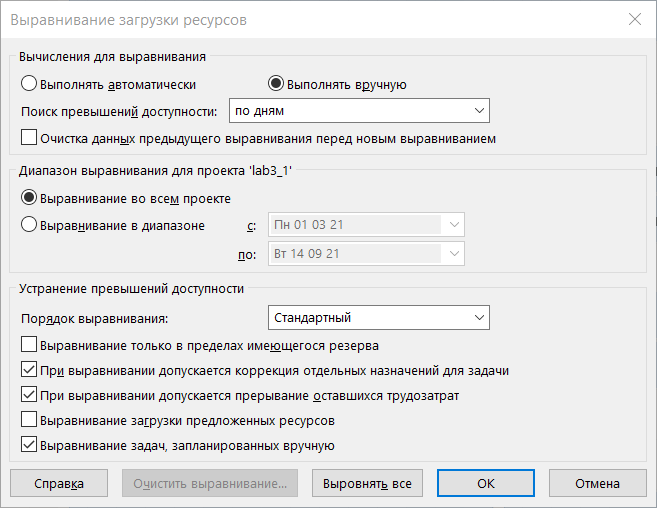
\includegraphics[width=0.7\linewidth]{src/lab3_1_1}
	\caption{Выравнивание}
	\label{fig:lab311}
\end{figure}

В результате выравнивания перегрузка ресурсов была устранена.

\section{Задание 2}
Подзадачи:
\begin{enumerate}
	\item отразите в плане проекта проведение еженедельного совещания по
	средам с 10 до 11 утра \ref{fig:lab321}
	\item привлеките к участию в совещании всех специалистов, кроме
	наборщиков данных и программистов №1 - 4 (их интересы на совещании
	представляет ведущий программист);
	\item устраните перегрузку ресурсов;
	\item в случае превышения бюджета и сроков реализации проекта проведите
	оптимизацию временных и финансовых параметров проекта.
\end{enumerate}

\begin{figure}[h]
	\centering
	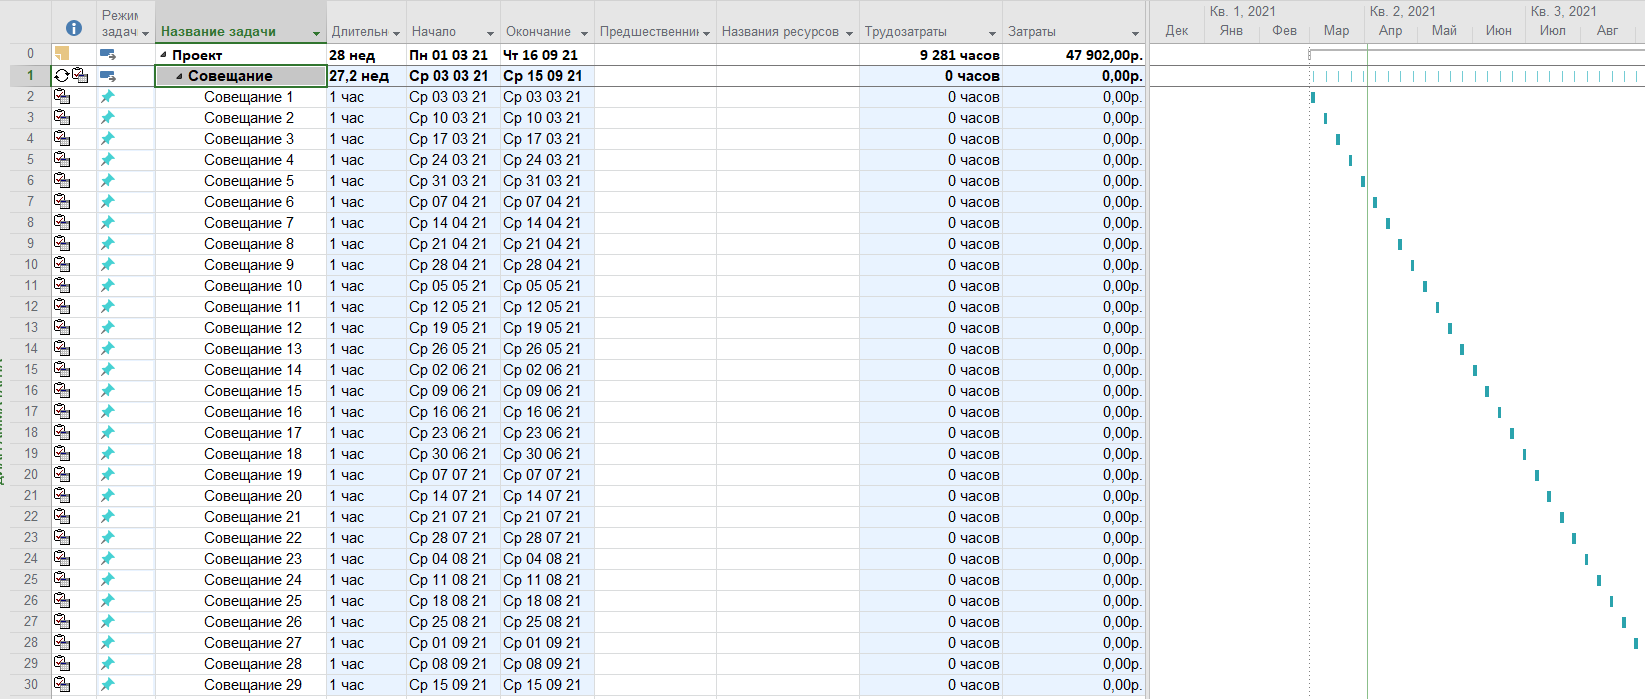
\includegraphics[width=0.7\linewidth]{src/lab3_2_1}
	\caption{Совещание}
	\label{fig:lab321}
\end{figure}

После добавленя совещания, появилась перегрузка ресурсов.
Так как ресурс не может одновременно быть на совещании и работать над задачами.











